\documentclass[../main.tex]{subfiles}

\begin{document}

\problem{3}

The following equation can be used to calculate thrust from the SSME:

\[
    Thrust = \dot{m} u_{exit} + \left({p_{exit}-p_{ambient}}\right) A_{exit}  
\]

\givens{}
\(A_{inlet} = 0.21\,\unit{\meter\squared}\)\\
\(A_{throat} = 0.054\,\unit{\meter\squared}\)\\
\(A_{exit} = 4.17\,\unit{\meter\squared}\)\\
\(p_0 = 20.408\,\unit{\mega\pascal}\)\\
\(T_{inlet} = 3600\,\unit{\kelvin}\)\\
\(\gamma=1.2\)\\
\(R=287\,\unit{\joule/\kilogram\cdot\kelvin}\)

\assumptions{}
The nozzle is choked and isentropic throughout the duration.

\problempart{a}

Plot the thrust of the SSME as a function of altitude from sea level to \(20 \, \unit{\kilo\meter}\) above sea level.
Include markers where the nozzle flow is under-expanded, over-expanded, and at design conditions (aerodynamically speaking).
The following equation can be used to calculate ambient pressure:

\[
    p_{ambient} = 101325 (1 - (2.25577 \cdot 10^{-5} \cdot h))^{5.25588}
\]

where \(h\) is height (in meters) above sea level. 

\solution{}

Given the SSME thrust equation, the parameters of interest for the problem are:

\begin{itemize}

    \item \(\dot{m}\)
    \item \(u_{exit}\)
    \item \(p_{exit}\)
    \item \(p_{ambient}\)
    \item \(A_{exit}\)

\end{itemize}

Of these, only the exit area is given.

We begin with \(\dot{m}\).
Mass flow through a choked nozzle is given by the following equation:

\[
    \dot{m} = \frac{p_0 A^*}{\sqrt{T_0}} \sqrt{\frac{\gamma}{R} \left({\frac{2}{\gamma+1}}\right)^{\frac{(\gamma+1)}{(\gamma-1)}}}
\]

\(p_0\) is given, but \(T_0\) is unknown. 
Given \(A_{inlet}/A_{throat}\) and recognizing that the flow is sonic at the throat (i.e., \(A_{throat} = A^*\)), we can numerically solve the Area-Mach relation for the (subsonic) Mach number at the inlet to the nozzle.

\[
    {\left({\frac{A_{inlet}}{A^*}}\right)}^2
    =
    \frac{1}{M_{inlet}^2}
    {\left[{
        \frac{2}{\gamma+1}
        \left({1 + \frac{\gamma-1}{2}M_{inlet}^2}\right)
    }\right]}^{(\gamma+1)/(\gamma-1)}
\]

\[
    M_{inlet} = 0.1542
\]

With the inlet Mach number and static temperature we can use isentropic relations to solve for the total temperature in the nozzle.

\[
    T_0 = 3608.56 \, \unit{\kelvin}
\]

Substituting known values into the mass flow equation yields the SSME choked mass flow:

\[
    \dot{m} = 702.29\, \unit{\kilogram/\second}
\]

Next, we solve for \(p_{exit}\) and \(u_{exit}\).
Once again using the Area-Mach relation and a numerical solver, we utilize \(A_{exit}/A_{throat}\) to solve for the exit Mach number.

\[
    M_e = 4.704  
\]

Then, we can use isentropic relations to calculate \(p_e\) and \(T_e\).

\[
    p_e = 18555.9\, \unit{\pascal}  
\]

\[
    T_e = 1123.12\, \unit{\kelvin}  
\]

To calculate the exit velocity, we solve for the sonic velocity at the exit plane.

\[
    a_{e} = \sqrt{\gamma R T_{e}} = 621.95\,\unit{\meter/\second}  
\]

The exit velocity is now easily found.

\[
    u_{e} = M_{e} a_{e} = 2925.7\,\unit{\meter/\second}  
\]

The final piece of information required to calculate SSME thrust is \(p_{ambient}\).
Given the relation between ambient pressure and altitude we calculate ambient pressure at all altitudes between 0 and 20 \(\unit{\kilo\meter}\).
Figure \ref{p_vs_alt} shows the curve of pressure vs. altitude for the range of altitudes of interest.

\begin{figure}[h!]
    \centering
    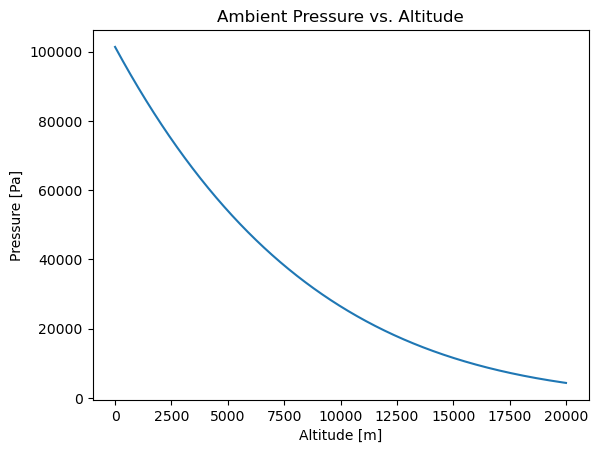
\includegraphics[scale=0.8]{../../images/problem_3/pamb_vs_alt.png}
    \caption{\(P_{amb}\) vs. Altitude}
    \label{p_vs_alt}
\end{figure}

Using the calculated ambient pressures we can finally calculate thrust at all points of interest.
Figure \ref{t_vs_alt} shows the SSME thrust vs. altitude curve between 0 and 20 \(\unit{\kilo\meter}\).
The SSME engine initially operates at an overexpanded condition, shown by the blue dotted line.
The design condition of the engine (where there are no shocks or expansions in the nozzle exhaust) comes at approximately \(h = 12236 \,\unit{\meter}\), with a design thrust of \(Thrust = 2054.7\,\unit{\kilo\newton}\), noted with a red star.
Beyond the design condition, the nozzle does not generate a sufficiently low static exit pressure value so the flow goes through expansion waves to reach equilibrium with the ambient pressure.
The underexpanded portion of the thrust curve is shown by the dashed orange line.

\begin{figure}[h!]
    \centering
    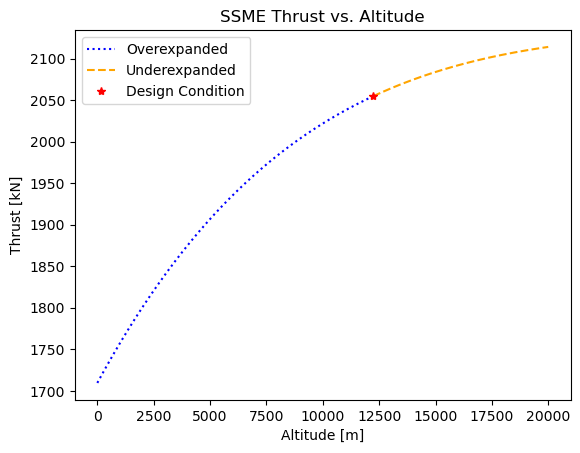
\includegraphics[scale=0.8]{../../images/problem_3/t_vs_alt.png}
    \caption{Thrust vs. Altitude}
    \label{t_vs_alt}
\end{figure}

\problempart{b}

Do you expect to see shock-diamonds or a plume when the space shuttle takes off?

\discussion{}

Because the SSME is initially overexpanded at takeoff, shock diamonds would be present in the exhaust of the SSME.
The low exit pressure from the nozzle goes through a series of oblique shocks to reach equilibrium with the ambient pressure, beginning a train of shock-diamonds that dissipate as the difference between exit pressure and ambient pressure shrinks at higher altitudes.

\problempart{c}

Does the ``design condition'' pertain to maximum thrust? Briefly explain.

\discussion{}

The design condition does not indicate the point of maximum thrust.
As shown in figure \ref{t_vs_alt}, the thrust continues to increase beyond the design point.
The key difference is that the thrust is less efficient outside of the design point, potentially limiting the vehicle's performance far away from the design condition.
The Space Shuttle did not fire the SSME at low altitudes, instead relying on the Solid Rocket Boosters (SRBs). 
The SRBs were designed to operate more efficiently at lower altitudes than the SSME which spent the majority of its time in flight at lower ambient pressures.


\end{document}

